\documentclass[a4paper, 11pt]{article}
\usepackage[margin=1in]{geometry} 
\usepackage[utf8] {inputenc}
\usepackage{amsmath,amssymb,amsthm}
\usepackage{mathtools}
\setlength{\parindent}{0cm}
\usepackage{graphicx,subfigure}
\usepackage{textcomp}
\usepackage{comment}
\usepackage{newunicodechar}
\usepackage{epstopdf}
\usepackage{caption}
\usepackage{lipsum}
\usepackage{float}
\usepackage{enumitem}
\usepackage{cellspace}
\usepackage{color}
\usepackage{textcomp}
\usepackage[hidelinks]{hyperref}
\usepackage{multirow}
\usepackage{siunitx}
\usepackage{algorithm}
\usepackage[noend]{algpseudocode}
\usepackage{tabularx}
\usepackage{booktabs}
\usepackage{titlesec}
\usepackage{pdfpages}
\usepackage{datetime}
\usepackage[autostyle]{csquotes}
\usepackage[usenames]{xcolor}
\usepackage{fancyhdr}
\pagestyle{fancy}
\setlength{\parindent}{0pt}
\usepackage{fontspec}
\defaultfontfeatures{Mapping=tex-text,Scale=MatchLowercase}
\setmainfont{Helvetica}

\let\svthefootnote\thefootnote

\rhead{
\includegraphics[height = 0.75cm]{Figures/AMZLogoRawRed.eps}}
\lhead{}

\titleformat{\section}
  {\normalfont\fontsize{18}{15}\bfseries}{\thesection}{1em}{}

\appto\normalsize{\belowdisplayshortskip=\belowdisplayskip}
\appto\small{\belowdisplayshortskip=\belowdisplayskip}
\appto\footnotesize{\belowdisplayshortskip=\belowdisplayskip}

\makeatletter
\renewcommand*\env@matrix[1][\arraystretch]{%
  \edef\arraystretch{#1}%
  \hskip -\arraycolsep
  \let\@ifnextchar\new@ifnextchar
  \array{*\c@MaxMatrixCols c}}
  \makeatother

\makeatletter
\def\BState{\State\hskip-\ALG@thistlm}
\makeatother

\begin{document}

\begin{titlepage}
	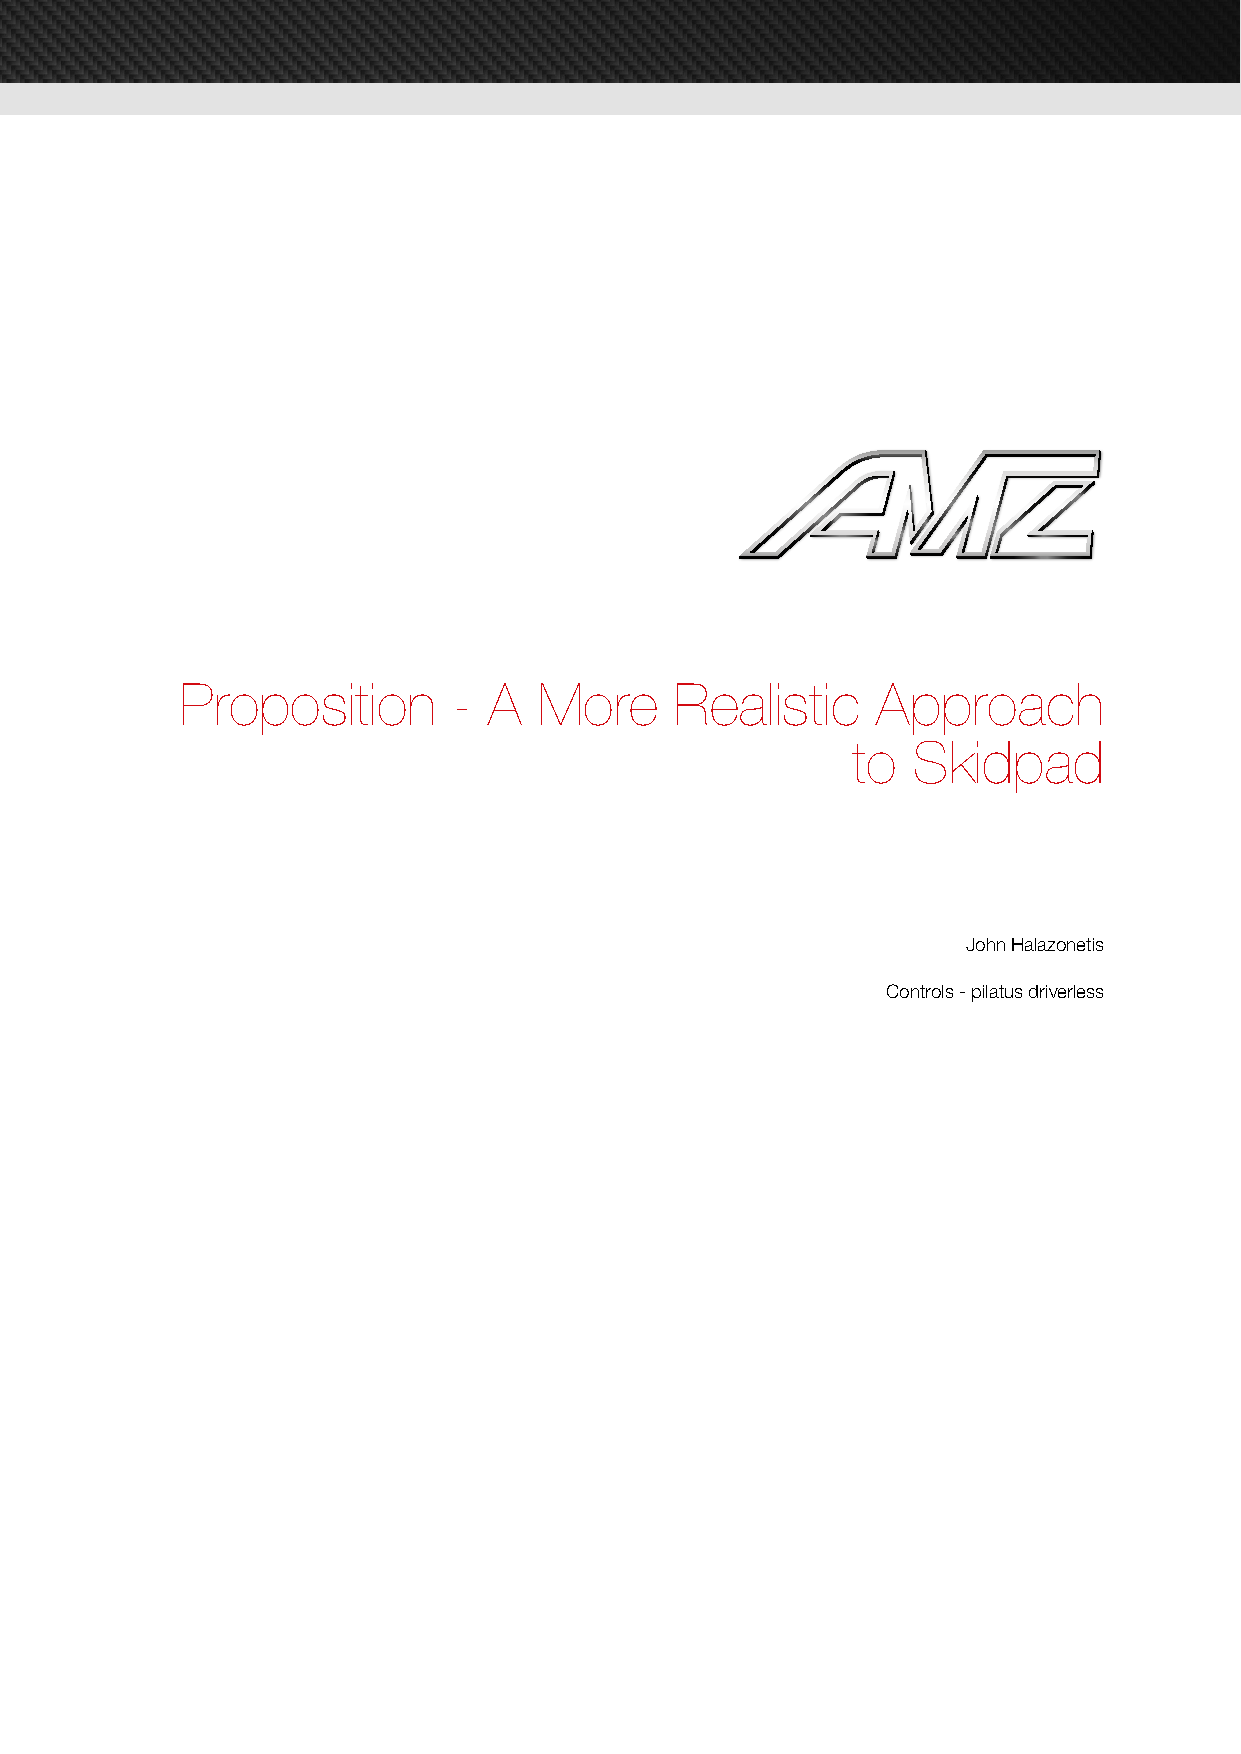
\includepdf{TitlePage.pdf}
\end{titlepage}

\newpage

\tableofcontents

\newpage

\section{Introduction}

The skidpad event is one of the four dynamic event in the Formula Student driverless competition, where the car is tested on its handling, traction and control capabilities. The primary objective for the teams is to complete the event in a minimum amount of time. The layout of the course is shown in Figure \ref{fig:SkidpadTrack}.

\section{Undertaking the Event}

As we can see in Figure \ref{fig:SkidpadTrack}, the track is the shape of a figure 8. The starting is situated towards the bottom arrow in Figure \ref{fig:SkidpadTrack} and will go into the clockwise turn on the right corner. After completing two rounds of the clockwise corner the car will turn into the counterclockwise corner located on the left. After completing two more rounds the vehicle will exit onto the straight at the top part of the circuit and stop within a specified distance.

\begin{figure}[H]
	\centering
	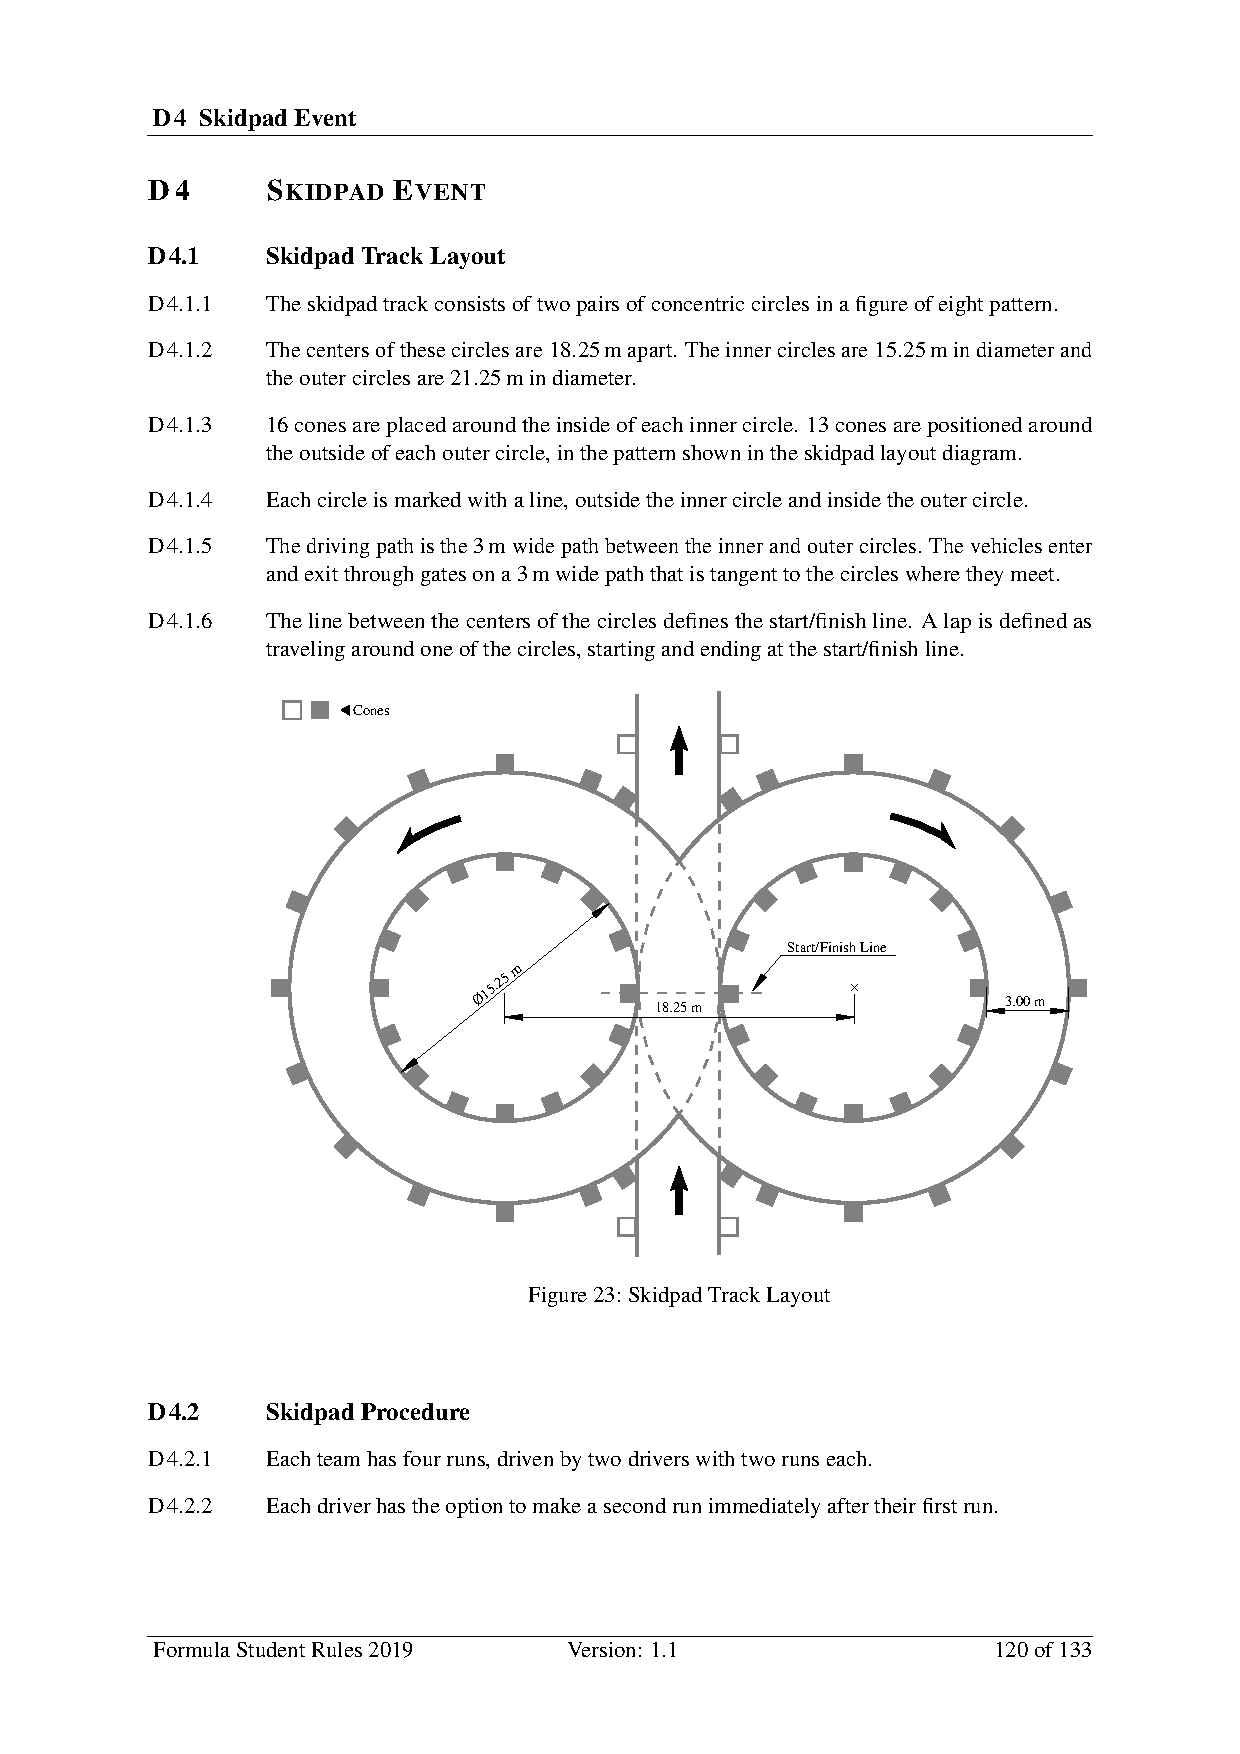
\includegraphics[trim = 4.5cm 8cm 2.5cm 11.5cm, clip, width = 0.8\textwidth]{Figures/SkidpadTrack}
	\caption{Skidpad course}
	\label{fig:SkidpadTrack}
\end{figure}

It is worth noting that only the second round of each of the respective clockwise and counter-clockwise corners will be timed and taken into account for awarding the points to the competing team.\\

Of course, in reality, the cones will not be placed exactly as in Figure \ref{fig:SkidpadTrack}. A safety margin will be defined due to this as well as the fact that the car may be able to place itself on the track with a great amount of precision.

\section{Determining the Optimal Trajectory}

In order to find the optimal trajectory for the purpose of this event, we will have to determine a path which maximizes the average speed of the the car \textit{on the second turn of the corner}, meaning a few things :
\begin{itemize}
	\item When the car is at steady state cornering conditions, the optimal radius is equal to the inner radius of corner (7.625 m) plus the rear track-width of the vehicle ($W_b$).
	\item When exiting the corner and moving onto either the counter-clockwise circle or the exiting the track the car should be allowed to accelerate as early as possible in order to increase its average speed (without losing grip and spinning out of course).
\end{itemize}

\subsection{Common and Simple Models}

A very simple initial trajectory can be found by taking the mean radius of the inside and outside track limits (middle line), and saying that the entry and exit trajectories are just straight lines (shown in Figure \ref{fig:SimpleTrajectory}). This can be used for a few rudimentary calculations and can give a good estimation on the time the car will take to complete the course, but there are a few subtleties that we ignore in this model that need our attention when applying this to a driverless vehicle.

\begin{figure}[H]
	\centering
	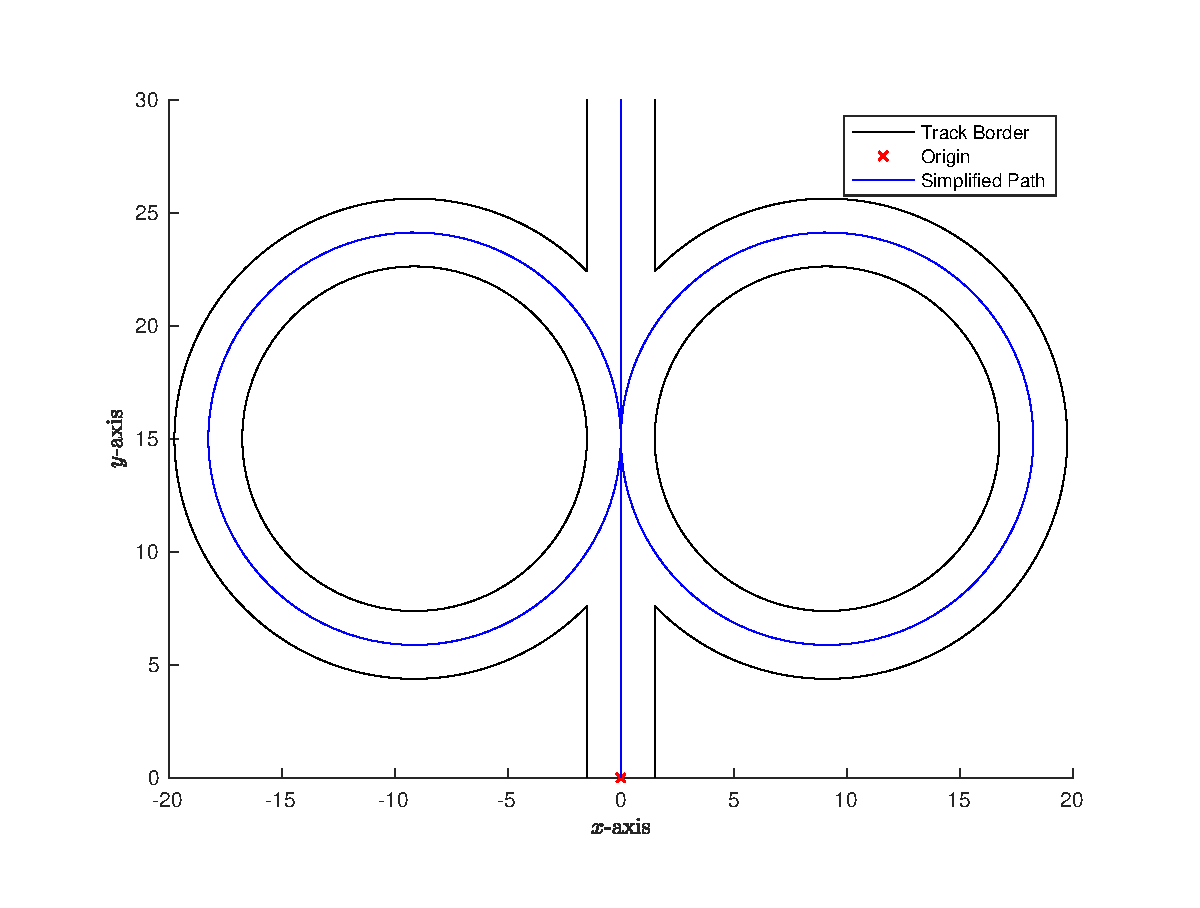
\includegraphics[trim = 1.5cm 0.8cm 1.5cm 1cm, clip, width = 0.7\textwidth]{Figures/SimpleTrajectory}
	\caption{ }
	\label{fig:SimpleTrajectory}
\end{figure}

\subsection{Transitioning Parts of the Event}

We define a transitioning phase when the cornering radius that the vehicle takes is no longer constant. In this particular event, we identify three transitioning phases. The first when the car starts the course and goes from the start straight into the first corner (located on the right side of the track) (Phase 1). The second is where the car exits the first corner (after having completed two turns) and goes into the second corner (phase 3), and the third is when the vehicle exits the second corner and heads toward the finishing line (phase 5). We can see a summary of all of the phases of skidpad in the list below :

\begin{table}[H]
	\centering
	\begin{tabular}{l l}
		Phase 1 : & Entry Phase\\
		Phase 2 : & Corner 1\\
		Phase 3 : & Transitioning phase from right to left circle of the course\\
		Phase 4 : & Corner 2\\
		Phase 5 : & Exiting Phase
	\end{tabular}
\end{table}

 We can see in this simplified model of the car's trajectory that the transitioning phases are almost non-existant, and therefore we have discontinuities for the steering and throttle control of the vehicle due to the first degree discontinuity of the cornering radius of the vehicle (which is also not very realistic). We can clearly see this when we represent the curvature (equal to $1/r$ where $r$ is the cornering radius of the corner) as a function of the distance travelled in Figure \ref{fig:CornerRadiusAFDistanceSimpleModel}.

\begin{figure}[H]
	\centering
	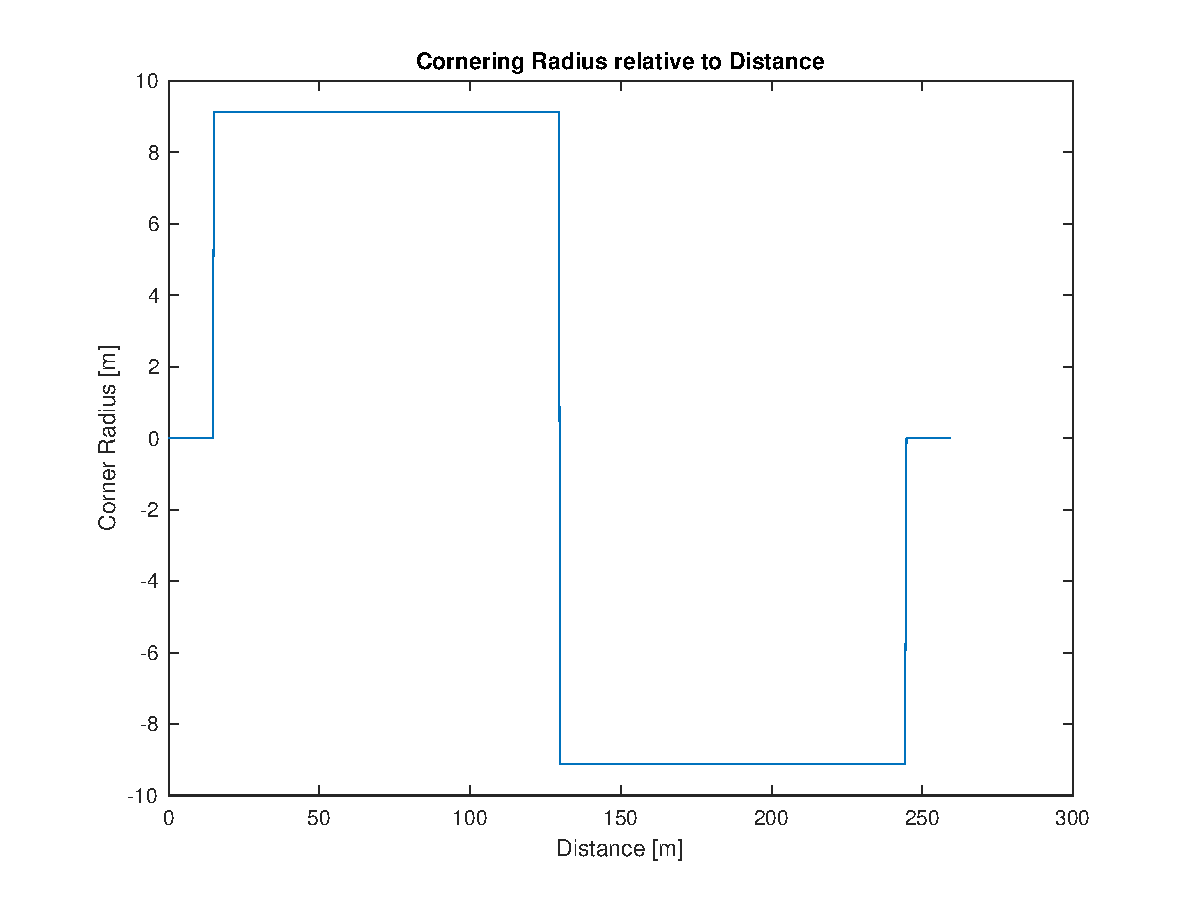
\includegraphics[width = 0.7\textwidth]{Figures/CornerRadiusDistance.eps}
	\caption{Curvature as a function of travelled distance}
	\label{fig:CornerRadiusAFDistanceSimpleModel}
\end{figure}

This makes it difficult to design a feedback controller for the steering and throttle inputs, because we are trying to follow a model with what is effectively step inputs. We will inevitably have some error at some point in the course that could be easily minimised or even neglected by taking a more realistic approach to the trajectory that the vehicle should follow.\\

\subsection{A More Realistic Approach of the Intended Trajectory}

In order to solve the aforementioned problem, we can introduce smooth curves to represent the vehicles trajectory when entering the first corner, transitioning from the first corner to the second, and exiting the second corner when heading for the finishing straight.\\

Before we begin, let us start by redefining the parts of the skidpad course. We now have seven parts that we will individually calculate and then stitch together in the software to make our trajectory :
\begin{enumerate}
	\item Starting straight
	\item Entering curve (into 1st corner)
	\item 1st corner (constant corner radius)
	\item Transitioning curve (from 1st corner to second)
	\item 2nd corner (constant corner radius)
	\item Exiting curve (out of 2nd corner)
	\item Finishing straight
\end{enumerate}

\subsubsection{Assumptions, Definitions and Other Details}
Assumptions :
\begin{itemize}
	\item The car will start at the middle of the starting straight.
	\item The car can end its course anywhere within the width if the exiting straight.
	\item The 1st and 2nd corners will be approximated to be perfect circles around the center points $\left(9.125\quad 15 \right)$ and $\left(-9.125\quad 15 \right)$.
\end{itemize}
\textbf{Definitions :}
\begin{itemize}
	\item We define a variable \texttt{TrackSafetyMargin} in our code. Since our control system will have a certain degree of precision of placing the car on the track, \texttt{TrackSafetyMargin} will be a length from the center of mass of the car to the track limits, in order to ensure that the car doesn't hit trespass the track limits.
	\item \texttt{InnerRadius} $=\frac{15.25}{2}$ (from figure \ref{fig:SkidpadTrack})
	\item \texttt{TrackWidth} $=3$ (from figure \ref{fig:SkidpadTrack})
	\item \texttt{InnerMarginRadius} = \texttt{InnerRadius} + \texttt{TrackSafetyMargin}
\end{itemize}



\subsubsection{Clothoids}

The entering curve, transitioning phase and exiting curve will be clothoids (also known as Euler spirals), since they are the ideal method for changing corner radius, they were the optimal choice for this application.

\begin{figure}[H]
	\centering
	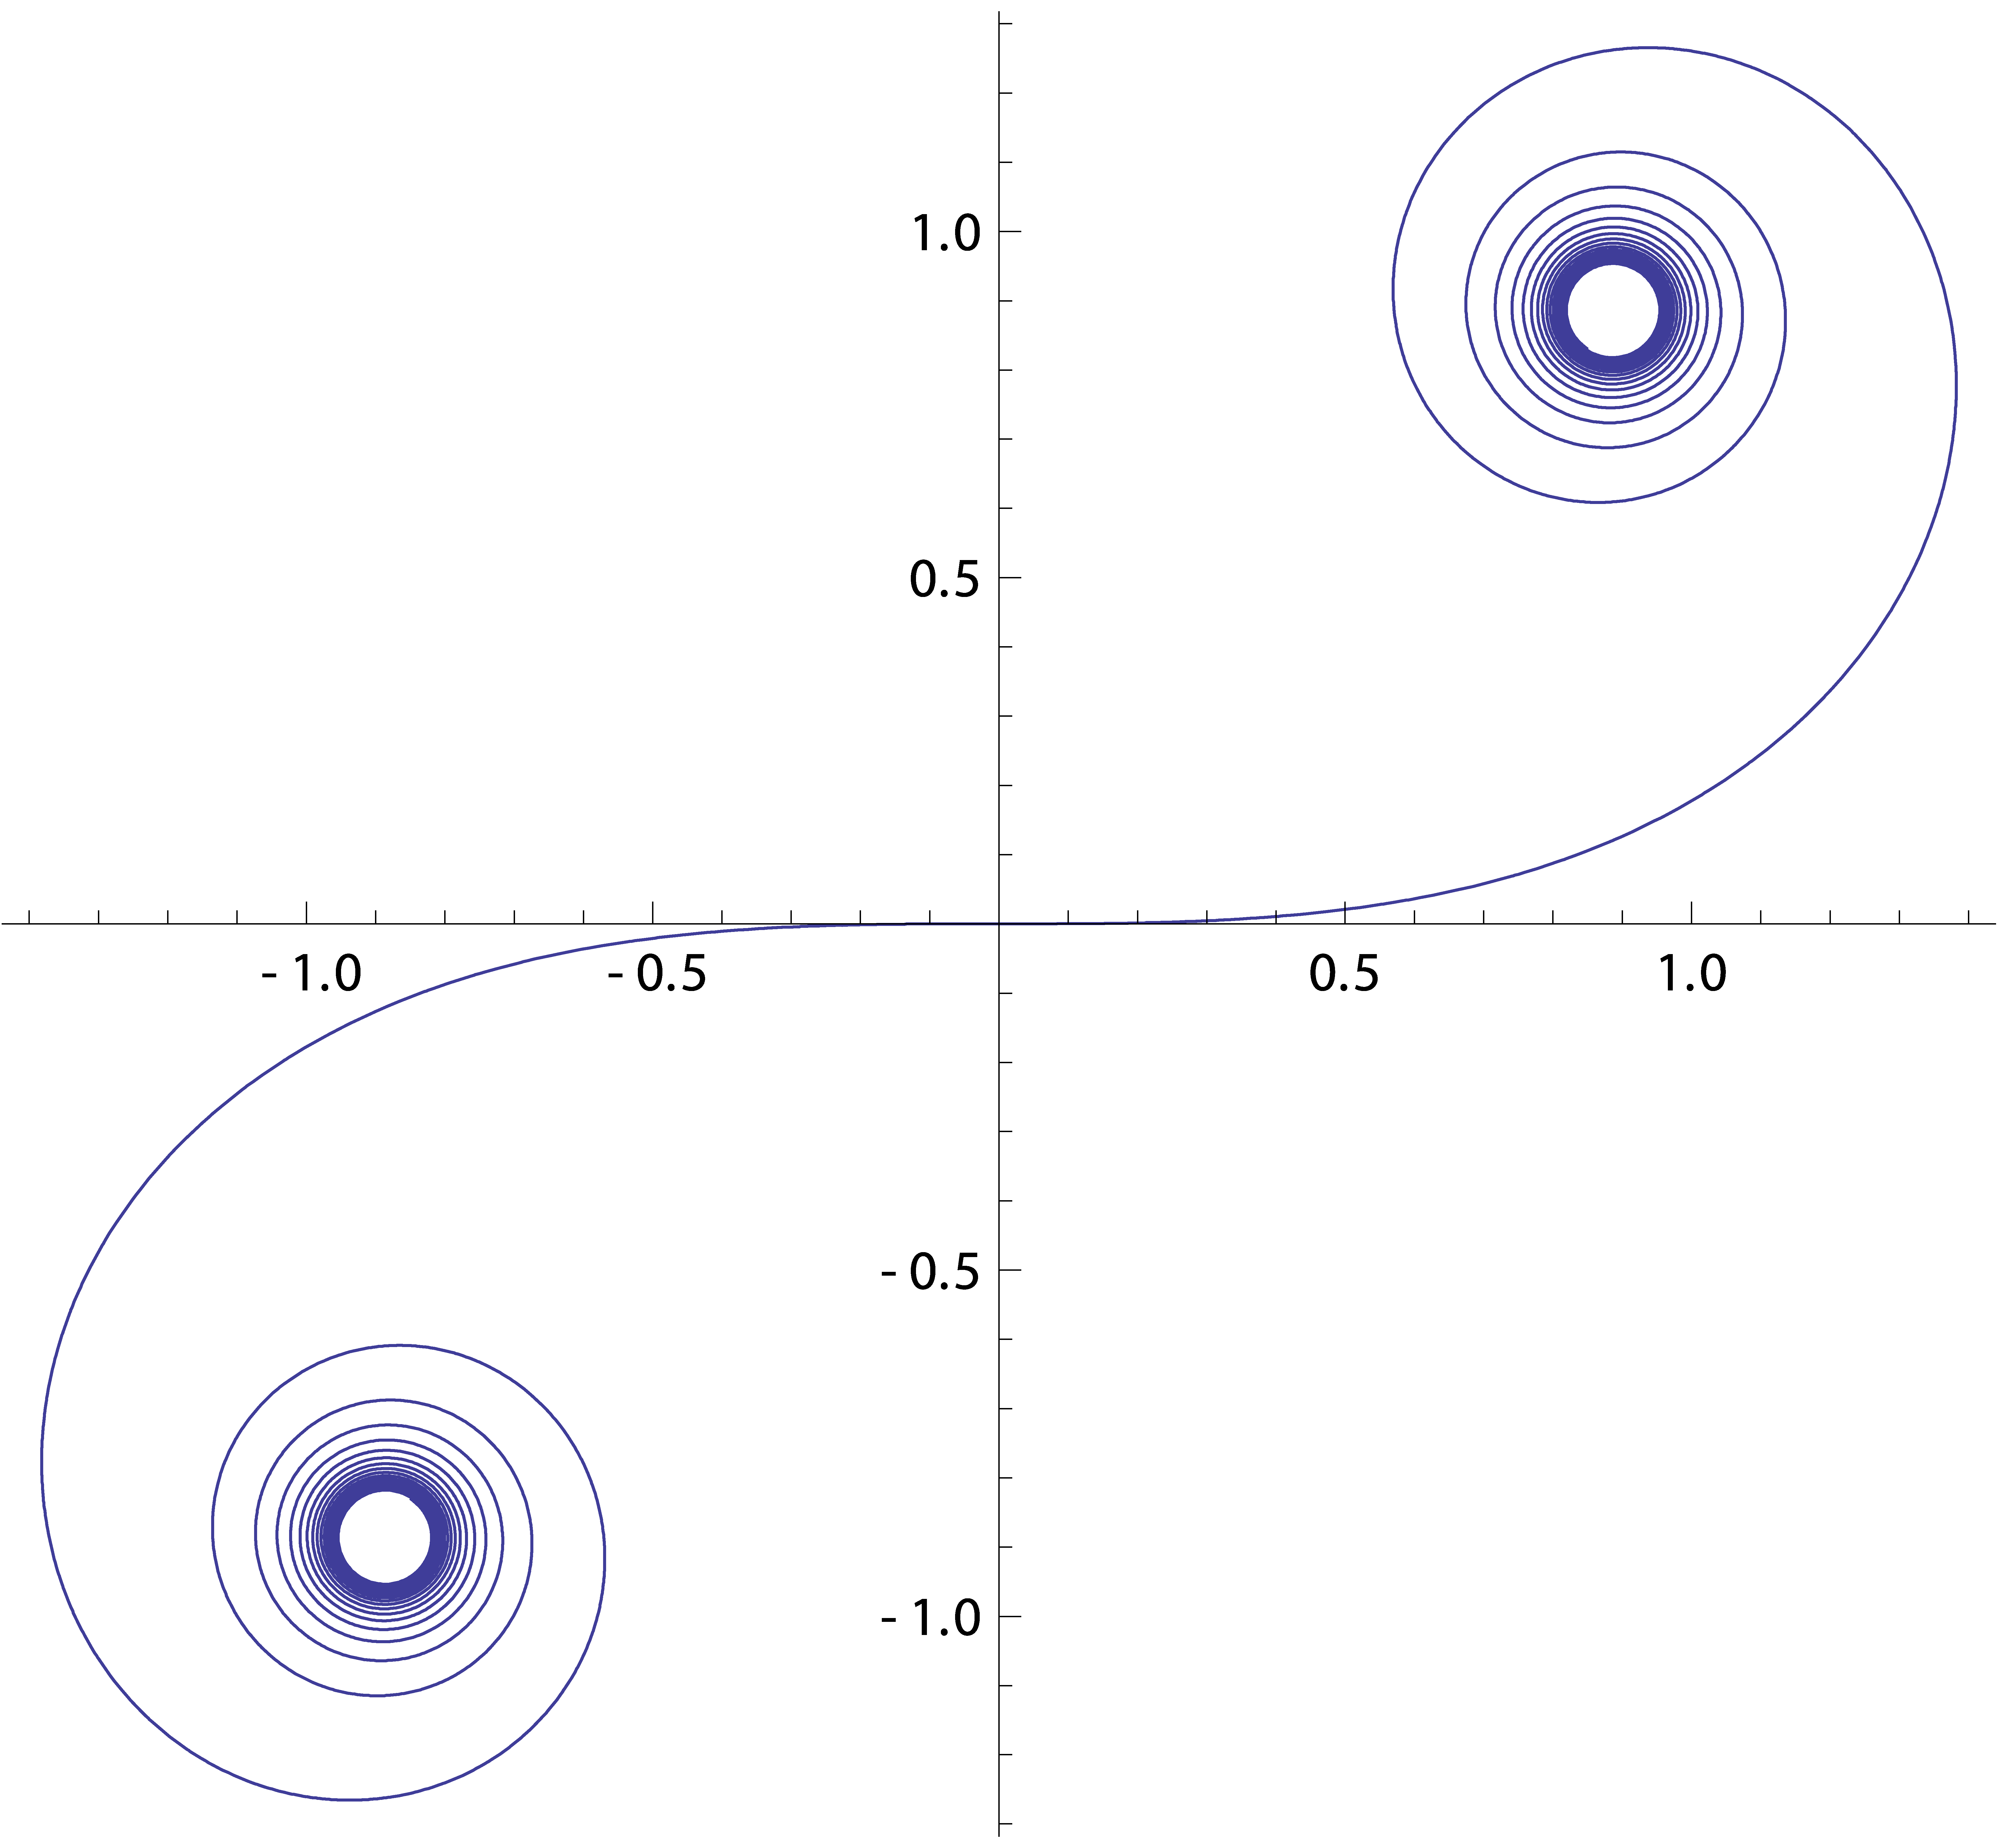
\includegraphics[width = 0.7\textwidth]{Figures/ClothoidExample.eps}
	\caption{A complete normalised clothoid}
	\label{fig:ClothoidExample}
\end{figure}

A few properties of this spiral are listed below in order to help with the understanding of the calculations to follow :
\begin{align*}
	&\text{Cartesian Parametrisation :} & x(t) &= a\int_0^t \cos\left(u^2 \right)du & y(t) &= a\int_0^t \sin\left(u^2 \right)du\\
	&\text{Cartesian Tangential Angle :} & \phi &= t^2\\
	&\text{Curvature Radius :} & R_c &= \frac{a}{2t}\\
	&\text{Curve length (as a function of $t$) :} & S &= a\cdot t
\end{align*}

We can now begin going through each part of the track and finding the clothoids that need to be applied.

\subsubsection{Part 1 : Starting Straight}
We need to calculate the length of the of the starting straight, however we need to know the parameters of the entering curve before we can do so.\\

$\hookrightarrow\quad$ See equation \ref{eq:StartStraightLengthResult} for the resulting equation.

\subsubsection{Part 2 : Entering Curve}
In order to find the clothoid, we need to find the scaling value $a_1$ and the angle at which the clothoid should end, $\theta_{j1}$. Since we know that $\theta_{j1} = t_{j1}^2$, we will just look for $a_1$ and $t_{j1}$.\\

Because we are joining a circle with a radius of \texttt{InnerMarginRadius}, at an angle of $t_{j1}^2$, we can start by finding $t_{j1}$ by calculating :
\begin{equation}
	\frac{18.25}{2} + \texttt{InnerMarginRadius}\cdot\left(1 - \cos\left(t_{j1}^2 \right) \right) =  2\cdot \texttt{InnerMarginRadius}\cdot t_{j1} \cdot \int_0^{t_{j1}} \sin\left(u^2 \right)du
\end{equation}

Now that we know $t_{j1}$, we can find $a_1$ :
\begin{equation}
	a_1 = 2 \cdot \texttt{InnerMarginRadius} \cdot t_{j1}
\end{equation}

We can also calculate the length of the clothoid :
\begin{equation}
	S_1 = a_1\cdot t_{j1}
\end{equation}

Now that we know the parameters of the first clothoid, we can find the length of the starting straight :
\begin{equation}
	\texttt{StartStraightLength} = 15 + \texttt{InnerMarginRadius}\cdot\sin\left(t_{j1}^2 \right) - a_1 \cdot \int_0^{t_{j1}} \cos\left(u^2 \right)du
	\label{eq:StartStraightLengthResult}
\end{equation}

When viewing the start straight and entering curve, we see :
\begin{figure}[H]
	\centering
	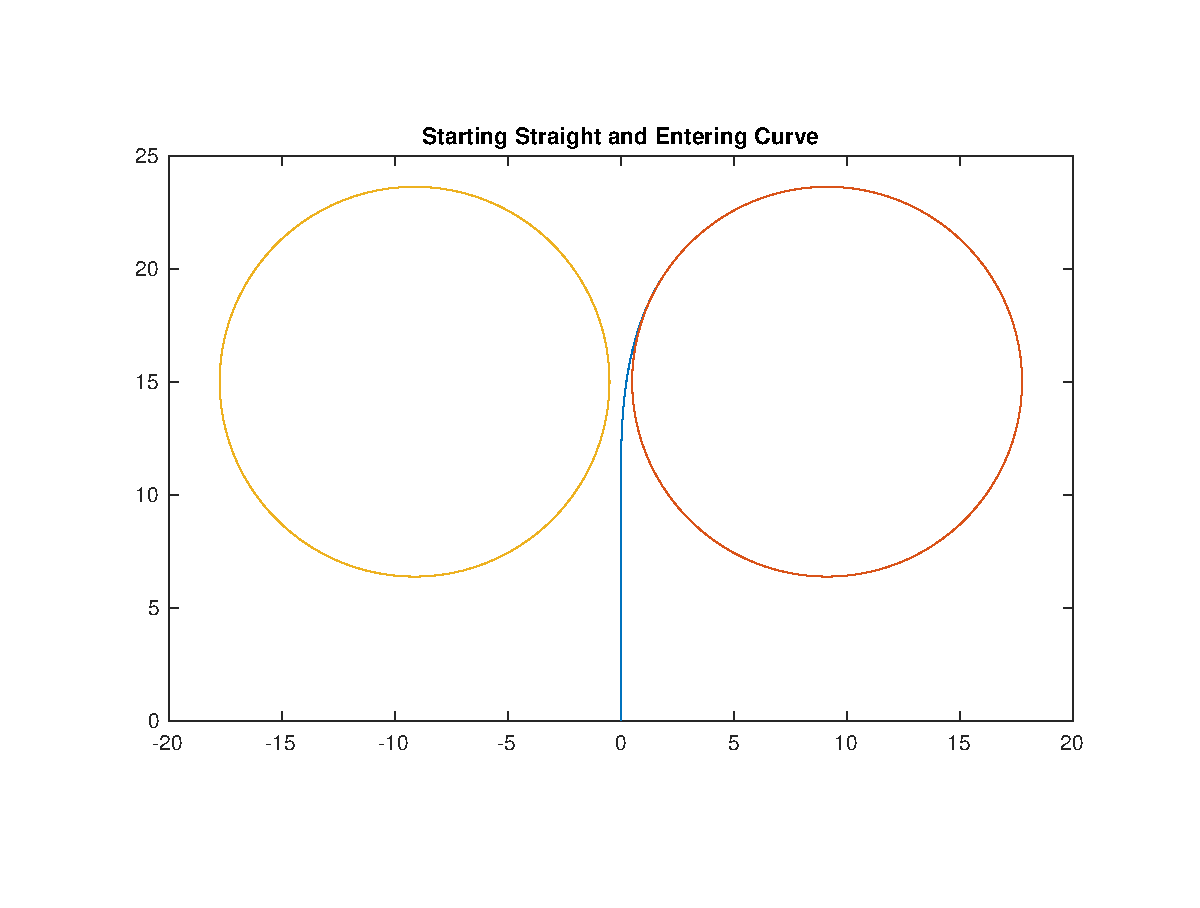
\includegraphics[trim = 1.9cm 2cm 1.3cm 1.5cm, clip, width = 0.7\textwidth]{Figures/StartStraightEnteringCurve.eps}
	\caption{ }
	\label{fig:StartStraightEnteringCurve}
\end{figure}

\subsubsection{Part 3 : 1st Corner}

We know that the first corner has a radius of \texttt{InnerMarginRadius} and starts at an angle of $t_{j1}^2$. However we do not know at what angle the car will exit the first corner, so we cannot calculate the length of the first corner yet. We need to find the value of the transitioning curve first.\\

$\hookrightarrow\quad$ See equation \ref{eq:Corner1Length} for the resulting equation.

\subsubsection{Part 4 : Transitioning Curve}
Based on the findings of \textit{A Note on Finding Clothoids} by D.S. Meek and D.J. Walton, we know that if we want to make a clothoid joining two curves, we can find the angle at which the clothoid joins the circles ($\theta_{j2}$) by solving the following :

\begin{equation}
	\frac{D^2}{4\cdot \texttt{InnerMarginRadius}^2} =  \left(\sqrt{\theta_{j2}}\cdot\int_0^{\theta_{j2}}\frac{\cos(u)}{\sqrt{u}}du  - \sin(\theta)\right)^2 +  \left(\sqrt{\theta_{j2}}\cdot\int_0^{\theta_{j2}}\frac{\sin(u)}{\sqrt{u}}du  + \cos(\theta)\right)^2
\end{equation}

Where $D$ is the distance between the center of the circles. For the skidpad, $D = 18.25$.

Since the clothoid is symmetrical around the origin point, we can now find the length of the 1st corner :
\begin{equation}
	\texttt{Corner1Length} = \texttt{InnerMarginRadius}\cdot\left(4\pi - \theta_{j1} - \theta_{j2} \right)
	\label{eq:Corner1Length}
\end{equation}

Also since we know $\theta_{j2} = \sqrt{t_{j2}}$, we can find the scaling factor $a_2$ as well as the length of the transitioning curve :
\begin{equation}
	a_2 = 2 \cdot \texttt{InnerMarginRadius} \cdot t_{j2}
\end{equation}
\begin{equation}
	S_2 = 2 \cdot a_2 \cdot t_{j2}
\end{equation}

However we still need to orient the curve in the 2D plane. We do this by finding the angle at which the curve needs to be in order be tangent with the circle.\\

If we draw a straight line that joins the ends of the curve (shown in purple in Figure \ref{fig:FindAngle}), and find the angle $\psi$ at which we need to rotate this line so that the end point touches the circle.

\begin{figure}[H]
	\centering
	\includegraphics[width = 0.6\textwidth]{Figures/FindAngle.eps}
	\caption{Clothoid that we need to rotate in blue, and circle to join is in yellow}
	\label{fig:FindAngle}
\end{figure}

We find angle $\phi$ simply by calculating the arctangent of the $x$ and $y$ coordinates at the end of the curve :
\begin{equation}
	\phi = \arctan\left(\frac{\int_0^{t_{j2}} \sin(u)du}{\int_0^{t_{j2}} \cos(u)du} \right)
\end{equation}

The length $L$ is found by using the Pythagoras theorem :
\begin{equation}
	L^2 = \left(\int_0^{t_{j2}} \sin(u)du \right)^2 + \left(\int_0^{t_{j2}} \cos(u)du \right)^2
\end{equation}

The angle $\delta$ is found by using the cosinus theorem for triangles :
\begin{equation}
	\delta = \arccos\left(\frac{9.125^2 + L^2 - \texttt{InnerMarginRadius}^2}{2\cdot 9.125\cdot L} \right)
\end{equation}

Finally, the angle $\psi$ is found :
\begin{equation}
	\psi = \frac{\pi}{2} - \delta - \phi
\end{equation}

Then we know the angle that we have to rotate the clothoid, and we can apply a rotation matrix to the $x$ and $y$ coordinates. After applying the correct rotation to our matrix, and drawing both ends of our clothoid, we will see the following when viewing our transition phase :
\begin{figure}[H]
	\centering
	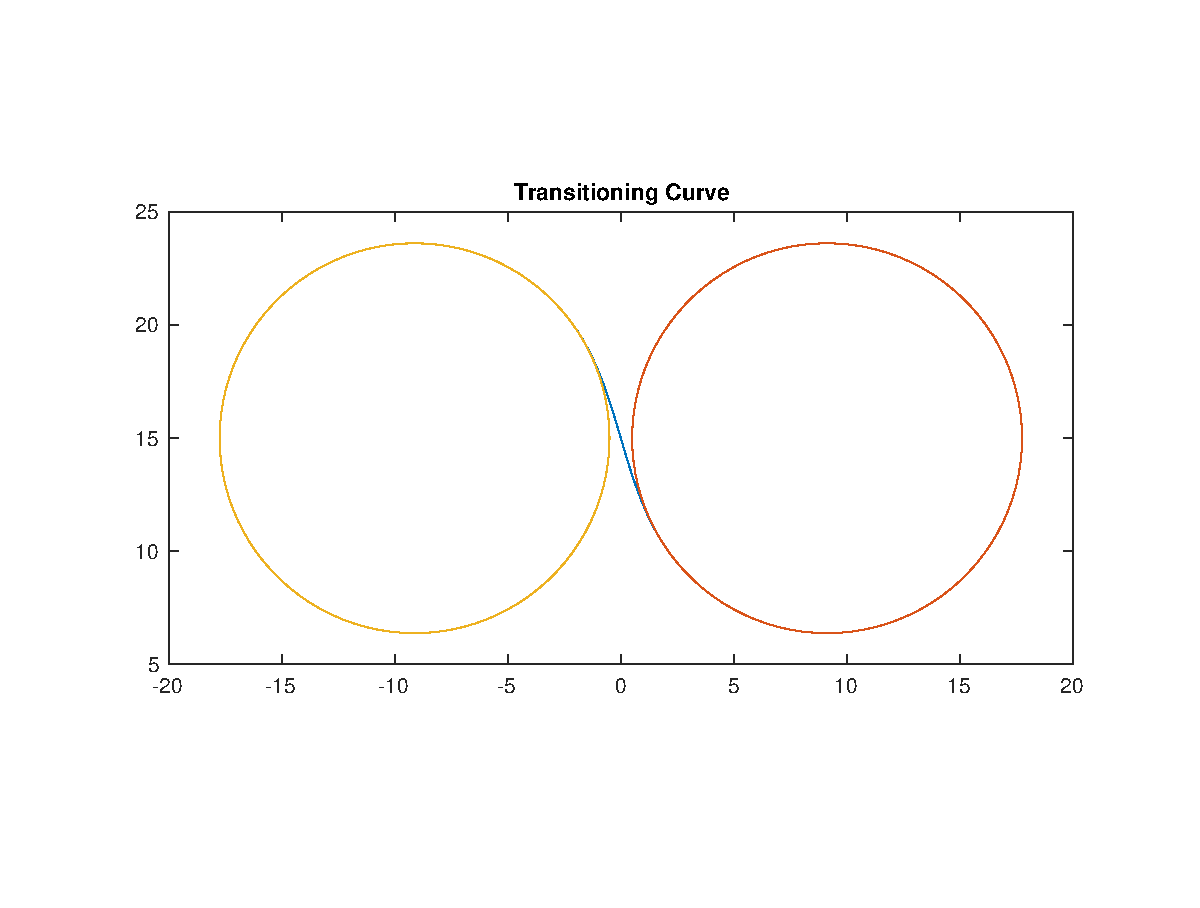
\includegraphics[trim = 1.5cm 3cm 1cm 2.5cm, clip, width = 0.7\textwidth]{Figures/TransitionCurve.eps}
	\caption{ }
\end{figure}

\subsubsection{Part 5 : Second Corner}

Similarly to the first corner, we approximate this to being a perfect circle. We cannot calculate the total length until we know the angle at which the exiting curve joins the 2nd corner.\\

$\hookrightarrow\quad$ See equation \ref{eq:Corner2Length} for the resulting equation.

\subsubsection{Part 6 : Exiting Curve}

The exiting curve is calculated in a very similar way to the entering curve. First we decide whether we wan the car to carry as much speed through the corner as possible (and get as close as it is allowed to the track limits). We switch this feature on or off by using the boolean variable \texttt{ExitMax}. We can then find the value of $t_{j3}$ :
\begin{itemize}
	\item If \texttt{ExitMax} is on, then we use the formula below to find $t_{j3}$ :
		\begin{align}
			\frac{\texttt{TrackWidth}}{2} - \texttt{TrackSafetyMargin} + \frac{18.25}{2} + \texttt{InnerMarginRadius}\cdot\left(1 - \cos\left(t_{j1}^2 \right) \right) =\nonumber \\ = 2\cdot \texttt{InnerMarginRadius}\cdot t_{j1} \cdot \int_0^{t_{j1}} \sin\left(u^2 \right)du
		\end{align}
	\item If \texttt{ExitMax} is off, then we use the formula below to find $t_{j3}$ :
		\begin{equation}
			\frac{18.25}{2} + \texttt{InnerMarginRadius}\cdot\left(1 - \cos\left(t_{j3}^2 \right) \right) =  2\cdot \texttt{InnerMarginRadius}\cdot t_{j3} \cdot \int_0^{t_{j3}} \sin\left(u^2 \right)du
		\end{equation}
\end{itemize}

Now that we know the value of $t_{j3}$, we can find the length of the second corner :

\begin{equation}
	\texttt{Corner2Length} = \texttt{InnerMarginRadius}\cdot\left(4\pi - \sqrt{t_{j2}} - \sqrt{t_{j3}} \right)
	\label{eq:Corner2Length}
\end{equation}

Now that we know the value of $t_{j3}$, we can also find the value of $a_3$ :
\begin{equation}
	a_3 = 2 \cdot \texttt{InnerMarginRadius} \cdot t_{j3}
\end{equation}

And hence the length of the exiting curve :
\begin{equation}
	S_3 = a_3\cdot t_{j3}
\end{equation}

\subsubsection{Part 7 : Finishing Straight}

Finally, we can find the length of the finishing straight from the exiting curve :
\begin{equation}
	\texttt{FinishStraightLength} = 15 + \texttt{InnerMarginRadius}\cdot\sin\left(t_{j3}^2 \right) - a_3 \cdot \int_0^{t_{j3}} \cos\left(u^2 \right)du
\end{equation}

The position on the $x$-axis will depend on whether \texttt{ExitMax} is activated or not.\\

When viewing the exiting curve and finishing straight, we see :
\begin{figure}[H]
	\centering
	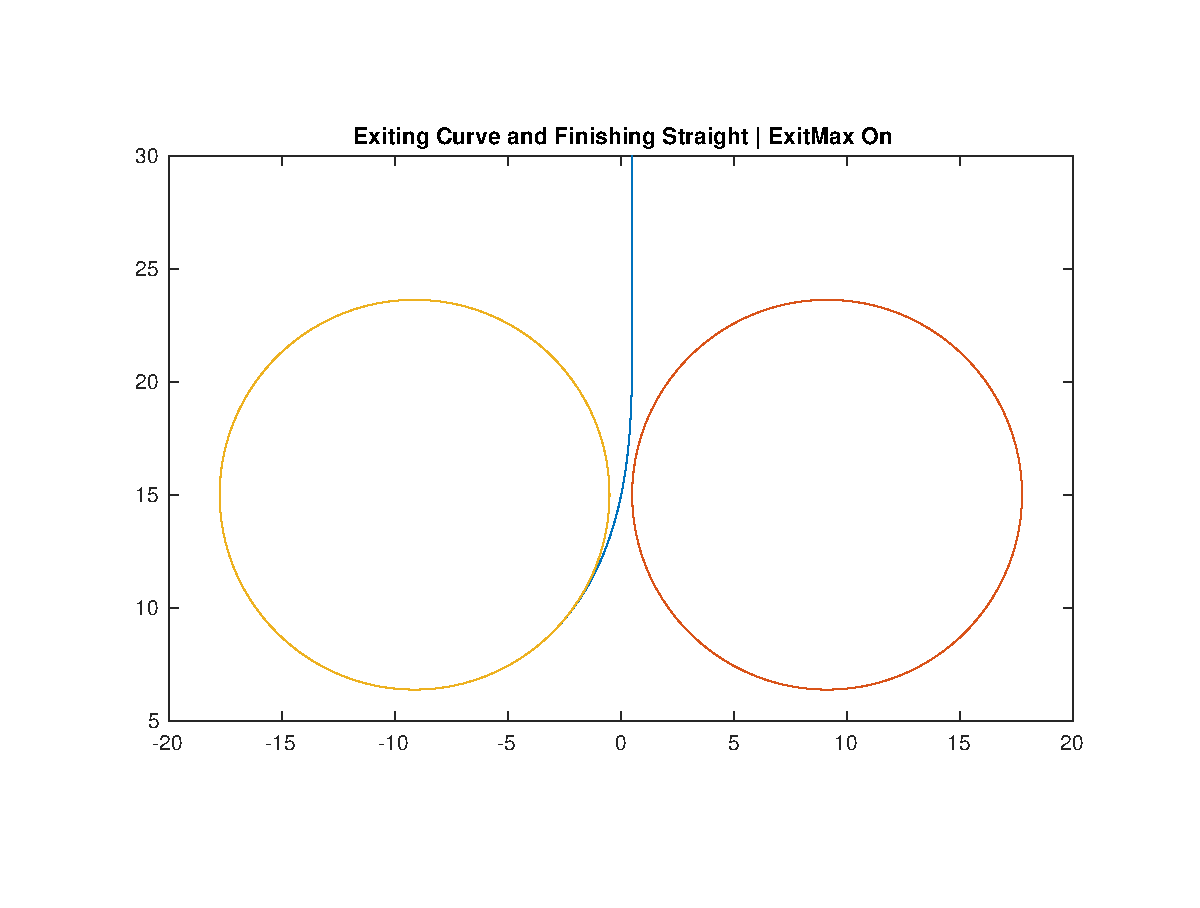
\includegraphics[trim = 2cm 2cm 1.5cm 1.8cm, clip, width = 0.7\textwidth]{Figures/ExitCurveFinishStraight}
\end{figure}

\subsection{Results}

We can then stitch these results together, and we obtain a more realistic trajectory for the skidpad event, on the left of Figure \ref{fig:SkidpadResultNoExitMax} we see the trajectory, and on the right we see the curvature:

\begin{figure}[H]
	\centering
	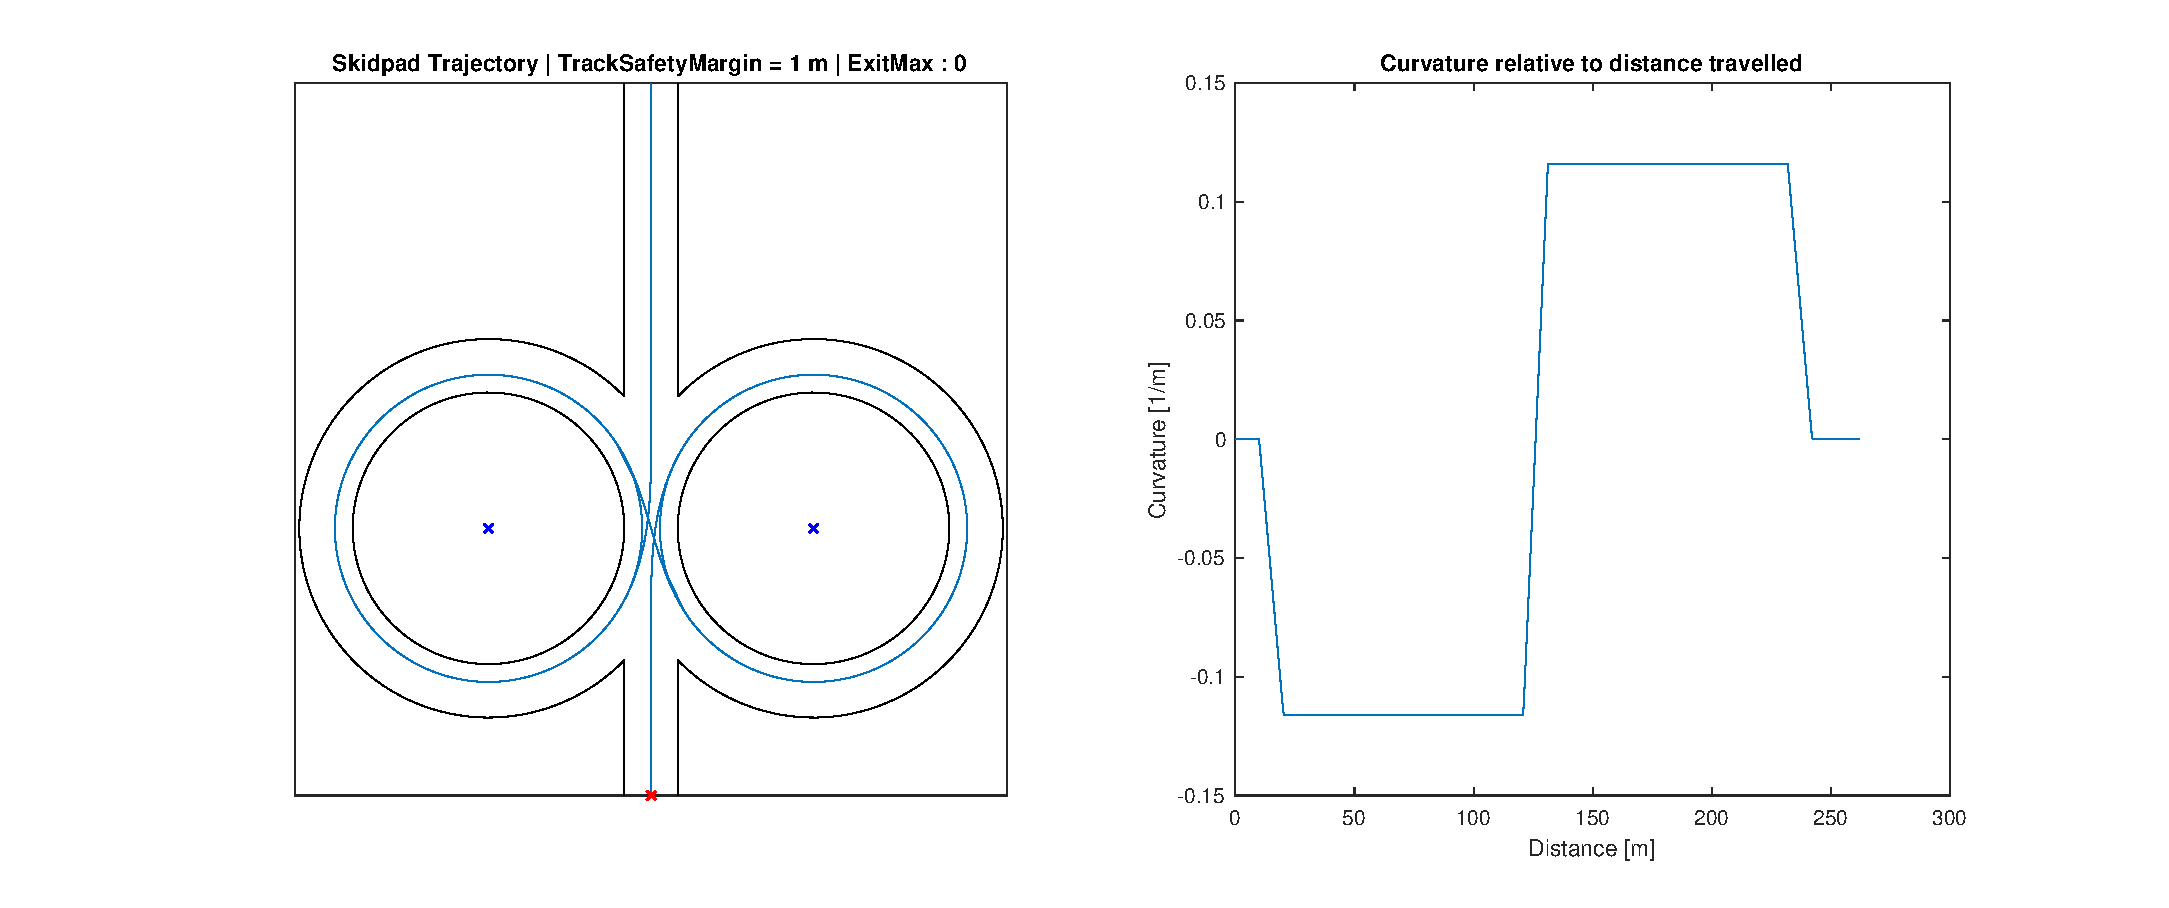
\includegraphics[trim = 4.5cm 0.5cm 3.1cm 0.6cm, clip, width = \textwidth]{Figures/SkidpadResultNoExitMax}
	\caption{ }
	\label{fig:SkidpadResultNoExitMax}
\end{figure}

We can see that when the variable \texttt{ExitMax} is off, the car will exit towards the center, however when it is activated, the car will be allowed to take as wide a line as possible, increasing the speed it can take through the corner. Similarly to Figure \ref{fig:SkidpadResultNoExitMax}, we see the trajectory on the left and the curvature on the right :

\begin{figure}[H]
	\centering
	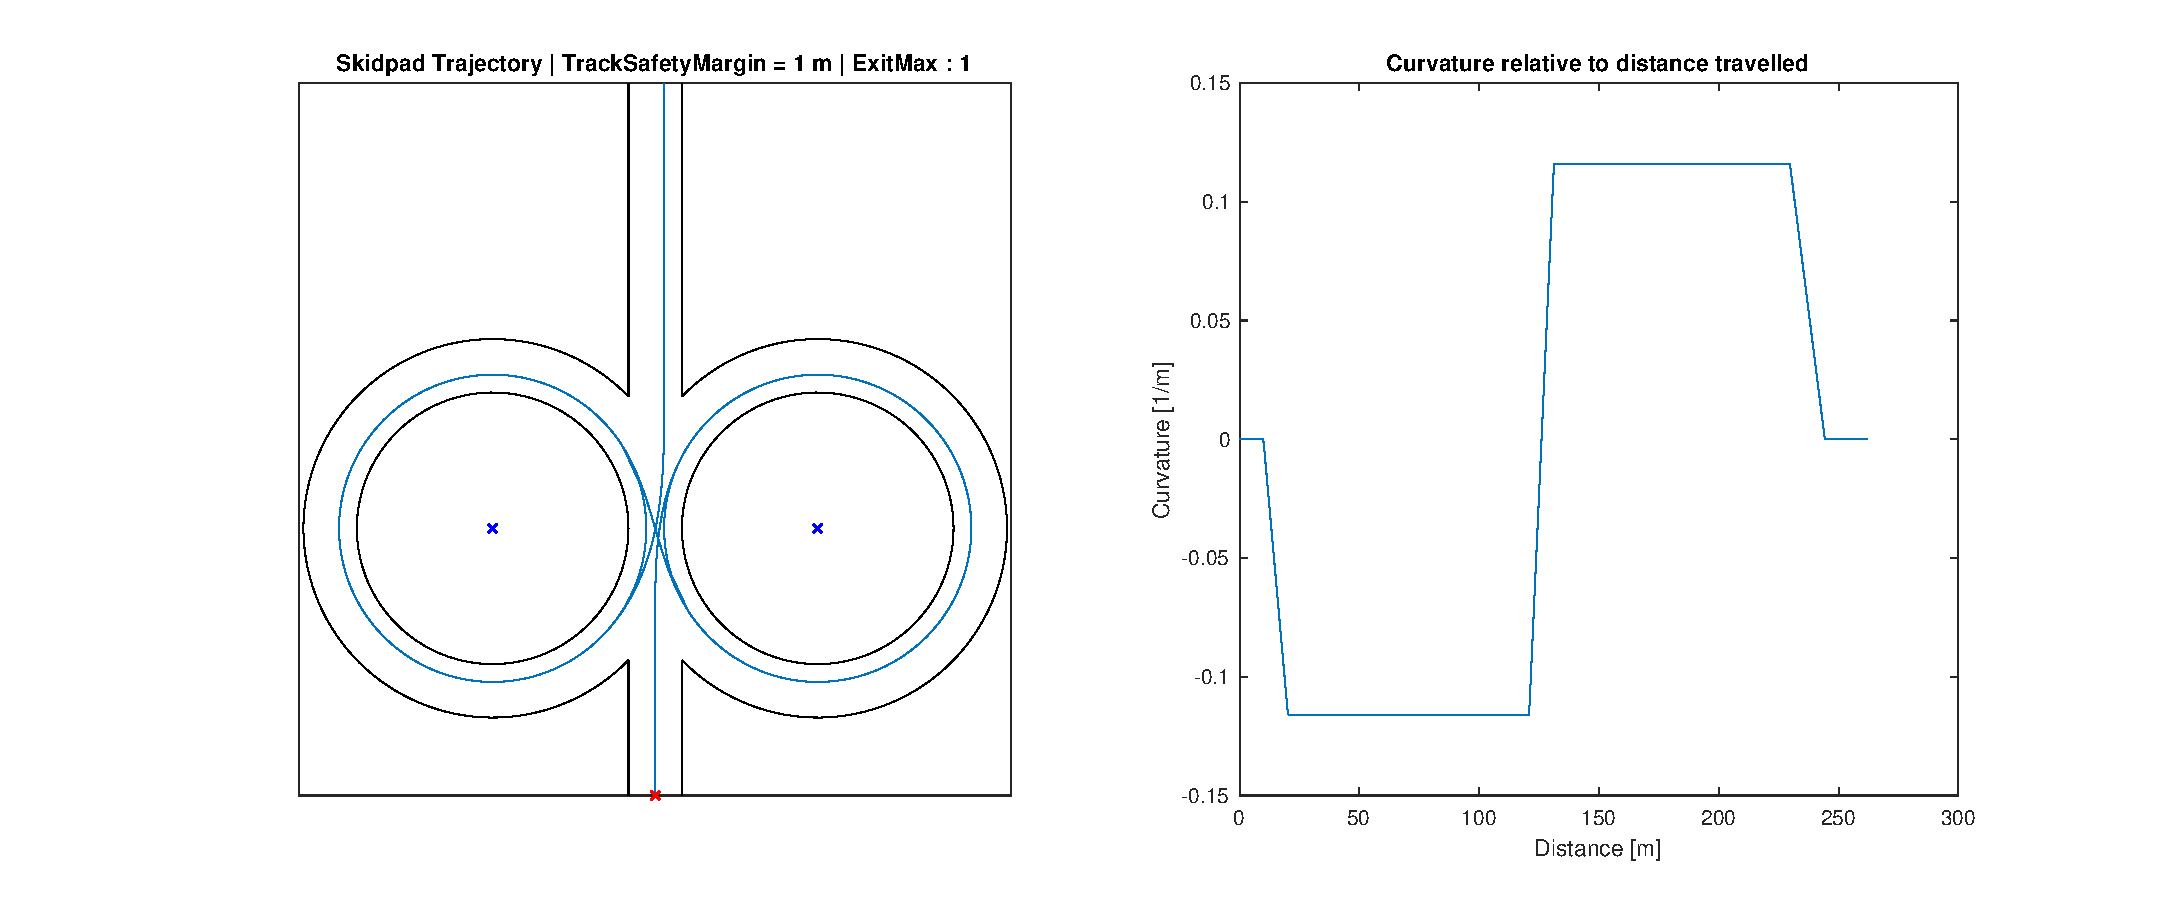
\includegraphics[trim = 4.5cm 0.5cm 3.1cm 0.6cm, clip, width = \textwidth]{Figures/SkidpadResultExitMax}
	\caption{ }
	\label{fig:SkidpadResultExitMax}
\end{figure}

In conclusion, we can see that we now have a first degree continuity when viewing the curvature over the course of the distance travelled. When the boolean \texttt{ExitMax} is activated, the slope of the curvature on the exit is less agressive, allowing for greater acceleration upon the exit of the last curve, increasing our average speed and hence decreasing the lap time.

\newpage
\section{Speed Trajectory}

Now that we have found the path for the car to follow, we need to determine the speed trajectory it should aim to follow over the course of the skidpad event. In order to do this, we will make use of the dynamic equations that govern the movement of the vehicle, whilst incorporating Pacejka's magic formula for slip angles. Throughout our calculations, we will make the following simplification assumptions :
\begin{itemize}
	\item Our car has 3 degrees of freedom
	\item Pacejka’s lateral tyre dynamics are simplified for pure lateral slip
	\item Longitudinal tyre dynamics are neglected
	\item Load transfers are neglected
\end{itemize}

\subsection{Method of Calculation}

In order to accurately predict the speed at each defined point of the track, we will need to build a small simulator. This simulator will follow the four simplification assumptions listed above. 

\subsubsection{Dynamics of the Vehicle}

We will use the following equations to describe the vehicle dynamics that are taken into account in this simplified model. We will then use these equations in the pseudo-code to explain how the algorithm of our basic simulator works. Tables \ref{tab:DynamicSymbols} and \ref{tab:DynamicIndices} show the nomenclature for the variables that will be used :
\begin{table}[H]
	\centering
	\begin{tabular}{r | l  l}
		$\alpha$ & Slip angle & [-]\\
		$v_x$ & Longitudinal velocity & [m/s]\\
		$v_y$ & Lateral velocity & [m/s]\\
		$\omega$ & Yaw rate & [rad/s]\\
		$\delta$ & Steering angle & [rad]\\
		$C_L$ & Aerodynamic lift coefficient & [-]\\
		$C_D$ & Aerodynamic drag coefficient & [-]\\
		$m$ & Mass & [kg]\\
		$W$ & Wheelbase & [m]\\
		$\rho$ & Air density & [kg/m$^3$]\\
		$A_w$ & Total wing area & [m$^2$]
	\end{tabular}
	\caption{Symbols used in dynamic equations}
	\label{tab:DynamicSymbols}
\end{table}

\begin{table}[H]
	\centering
	\begin{tabular}{r | l}
		$x$ & Longitudinal direction\\
		$y$ & Lateral direction\\
		$f$ & Front wheel\\
		$r$ & Rear wheel\\
		$CG$ & Center of gravity/mass\\
		$CP$ & Center of pressure
	\end{tabular}
	\caption{Indices used in dynamic equations}
	\label{tab:DynamicIndices}
\end{table}

One can also use Figure \ref{fig:TwoWheelModelTwoWheelSteerFourWheelDrive} to get a better representation of the vehicle.

\begin{figure}[H]
	\centering
	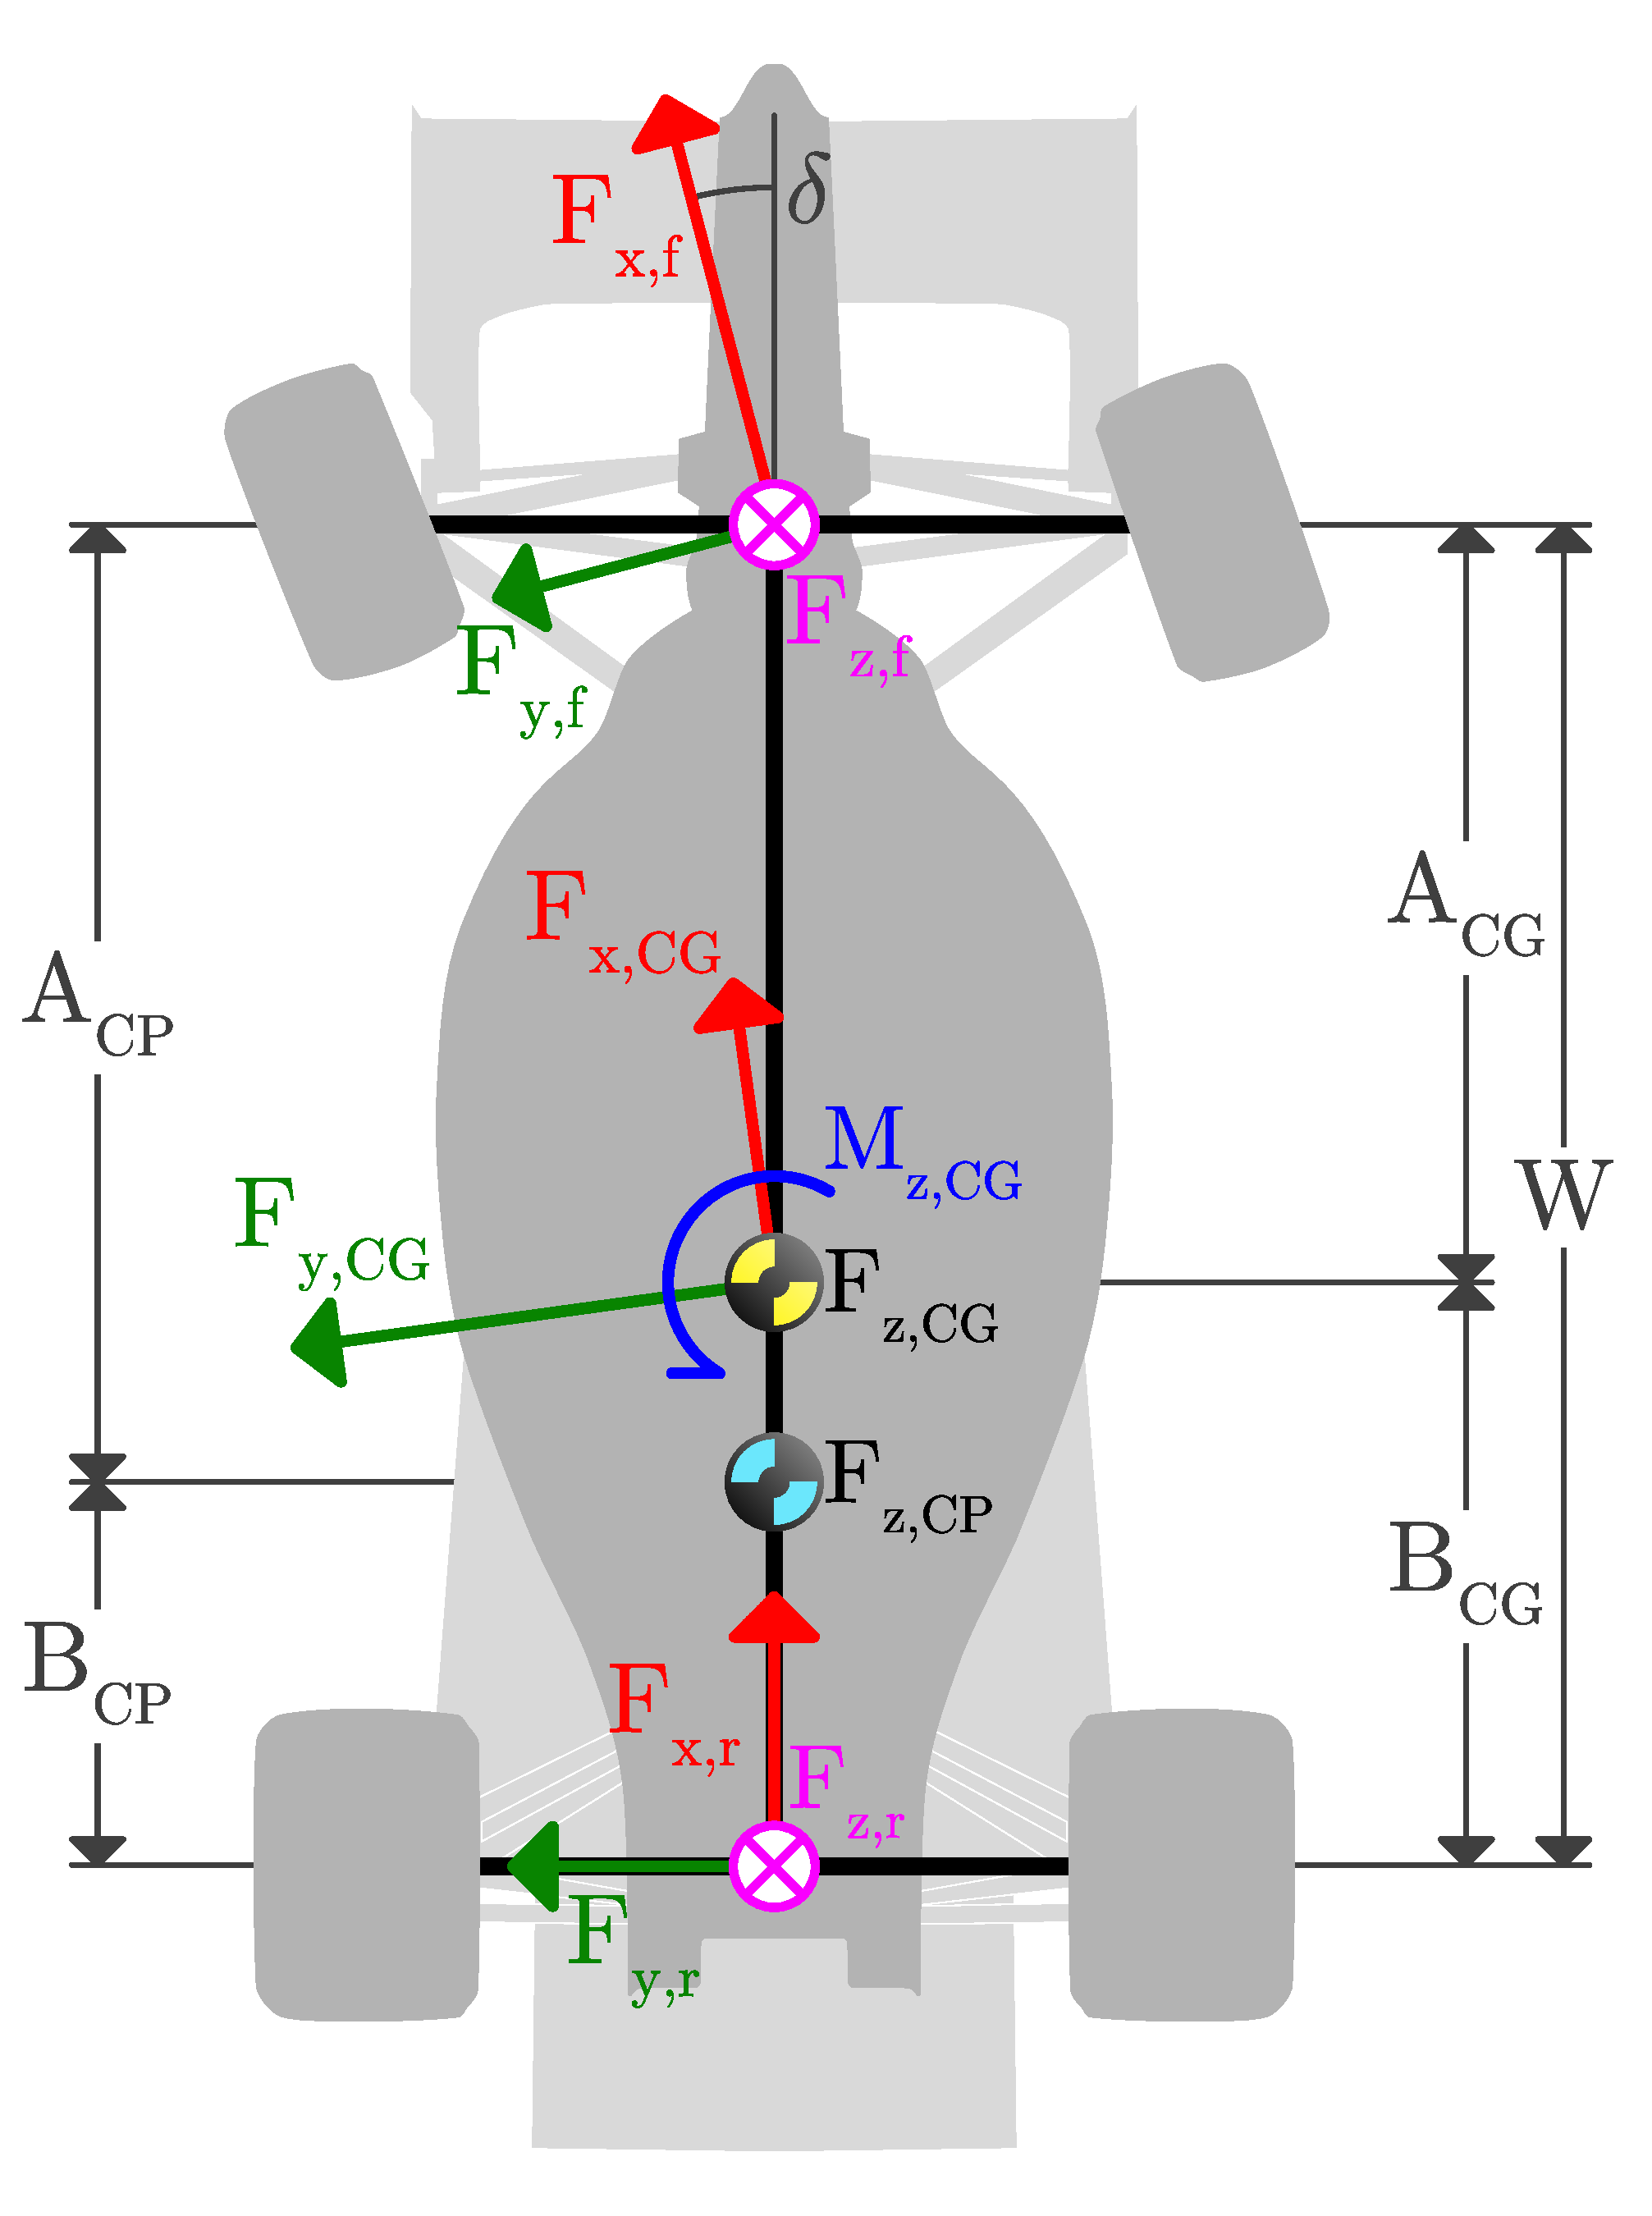
\includegraphics[width = 0.45\textwidth]{Figures/TwoWheelModelTwoWheelSteerFourWheelDrive.eps}
	\caption{Representation of the vehicle model we take with the forces annotated on each point where they are applied.}
	\label{fig:TwoWheelModelTwoWheelSteerFourWheelDrive}
\end{figure}

We can now start by listing the formulas of the forces, moments, angles, and geometrical relations that we will need for our algorithm.

\paragraph{Vertical Forces} ~\\
The total vertical force on each of the two wheels of our bicycle model is the sum of the weight and the aerodynamic downforce at a specific speed :
\begin{equation}
	F_{z,tot} = mg + \frac{1}{2}\rho A C_L v_x^2
	\label{eq:TotalNormalForce}
\end{equation}
For each wheel, we will have :
\begin{align}
	F_{z,f} &= \frac{B_{CG}}{W}\cdot mg + \frac{B_{CP}}{W}\frac{1}{2}\rho A C_L v_x^2\label{eq:FrontNormalForce}\\
	F_{z,r} &= \frac{A_{CG}}{W}\cdot mg + \frac{A_{CP}}{W}\frac{1}{2}\rho A C_L v_x^2\label{eq:RearNormalForce}
\end{align}

\paragraph{Slip Angles} ~\\
The slip angles for the front and rear tires are given by :
\begin{align}
	\alpha_f &= \arctan\left(\frac{\left(v_y + \omega\cdot A_{CG} \right)\cos(\delta) - v_x\sin(\delta)}{v_x\cos(\delta) + \left(v_y + \omega\cdot A_{CG} \right)\sin(\delta)} \right)\label{eq:FrontSlipAngle}\\
	\alpha_r &= \arctan\left(\frac{v_y + B_{CG}\cdot\omega}{v_x} \right)\label{eq:RearSlipAngle}
\end{align}

\paragraph{Lateral Forces} ~\\
If we know the speed of the vehicle $v$, we know that the lateral force on the center of mass of the vehicle can be easily found :
\begin{equation}
	F_{y,CG} = \frac{m\cdot v^2}{R_G}
	\label{eq:LateralForceCG}
\end{equation}

We can then easily find the instantaneous lateral forces on each of the wheels of our two wheel model by solving the system :
\begin{equation}
	\left\{\begin{matrix}
		F_{y,f}\cdot\cos\delta + F_{y,r} = F_{y,CG}\cdot\cos\theta_{CG}\\
		F_{y,f}\cdot\sin\delta = F_{y,CG}\cdot\sin\theta_{CG}
	\end{matrix} \right.
	\label{eq:LateralForcesSystem}
\end{equation}

The maximum lateral tire forces are given by the downforce on each wheel and the friction coefficient given by Pacejka's magic formula as a function of the slip angle of the respective wheel.
\begin{equation}
	F_{y,i} = F_{z,i}\cdot D_i\cdot\sin\left\{C_i\cdot\arctan\left[B_i\cdot\alpha_i\left(1-E_i \right) + E_i\cdot\arctan\left(B_i\cdot\alpha_i \right) \right] \right\}
	\label{eq:MaxLateralForce}
\end{equation}

\paragraph{Longitudinal Forces} ~\\
Now we need to determine the longitudinal force $F_{x,i}$ for each wheel $i$. We can independently calculate $F_{x,i}$ using Pacejka's magic formula :
\begin{equation}
	F_{x,i} = D_i\cdot\sin\left\{C_i\cdot\arctan\left[B_i\cdot\left(1-E_i \right)\cdot\alpha_i + E_i\arctan\left(B_i\cdot\alpha_i \right) \right] \right\}
	\label{eq:MaxLongForce}
\end{equation}

This formula is used however only if we have applied a longitudinal force to our tire. Since this is not the case, we will need to find another way to calculate $F_{x,i}$. Nevertheless, we will still need equation \ref{eq:MaxLongForce} in the near future.\\

For this event, we choose to model the maximum possible acceleration (and braking) of the car we are simulating without losing traction, this will obviously require the user to input the motor curves and braking force. We can also simulate moderate acceleration and braking, by simply multiplying these values by constant between 0 and 1.\\

We therefore want to find the value of $F_{x,i}$ for each wheel $i$ that puts the sum of $F_{y,i}$ and $F_{x,i}$ on the limit of the traction circle. As simple method to find $F_{x,i}$ when $F_{y,i}$ and $F_{x,i}$ are both non-zero is the elliptical approach :
\begin{itemize}
	\item Calculate $F_{y,i}$ and $F_{x,i}$ separately
	\item Cut down on $F_{x,i}$ so that the vector ($F_{y,i}$ $F_{x,i}$) doesn't exceed the maximum magnitude :
		\begin{equation}
			F_{x,i} = F_{x,i-\max}\cdot\sqrt{1-\left(\frac{F_{y,i}}{F_{y,i-\max}} \right)^2}
			\label{eq:LongitudinalForce}
		\end{equation}
		where:
		\begin{itemize}
			\item $F_{x,i}$ is the resulting combined slip longitudinal force
			\item $F_{x,i-\max}$ is the longitudinal force as calculated using equation \ref{eq:MaxLongForce}
			\item $F_{y,i}$ is the current lateral force calculated using the system \ref{eq:LateralForcesSystem}
			\item $F_{y,i-\max}$ is the maximum lateral force possible calculated from \ref{eq:MaxLateralForce}
		\end{itemize}
\end{itemize}

This method favors lateral forces over longitudinal ones (cuts down the longitudinal force and leaves $F_{y,i}$ intact).

\paragraph{General Equation of Movement} ~\\
In order to relate the sum of these forces onto the acceleration of center of mass of the vehicle, we use equation \ref{eq:GeneralMovement} to calculate the acceleration of the vehicle :
\begin{equation}
	F_{x,CG} - F_{drag} - C_{roll}\cdot m\cdot g = \left[\sum_{i=1}^{4}\left(\frac{J_{i,m}}{R_{i,w}^2}\cdot i_i^2 + \frac{J_{i,w}}{R_{i,w}^2} \right) + m \right]a
	\label{eq:GeneralMovement}
\end{equation}

For this equation, we use the following nomenclature :
\begin{table}[H]
	\centering
	\begin{tabular}{r | l  l}
		$F_{x,CG}$ & Propulsion force on center of gravity/mass & [N]\\
		$F_{drag}$ & Drag forces on the body of the vehicle & [N]\\
		$C_{roll}$ & Rolling resistance coefficient $i$ & [-]\\
		$R_{i,w}$ & Active radius of wheel $i$ & [m]\\
		$i_{i}$ & Transmission ratio on wheel $i$ & [-]\\
		$J_{i,m}$ & Inertia of electric motor on wheel $i$ & [kg$\cdot$m$^2$]\\
		$J_{i,w}$ & Inertia of wheel $i$ & [kg$\cdot$m$^2$]\\
		$m$ & Total mass of vehicle & [kg]\\
		$a$ & Acceleration of vehicle & [m$\cdot$ s$^{-2}$]
	\end{tabular}
\end{table}

Now that we have the equations that explain the dynamics of the car in place, we can now proceed with how our simulator's algorithm will work. We will start by solving the steady state cornering problem, and then finding the speed at the other points on the track by simulating the vehicle using the steady state speeds as boundary conditions.

\subsubsection{Solving the Steady State Cornering Problem}

From its definition, a steady state cornering condition implies that the total acceleration of the car is zero, and the the only accelerative forces that the car will exert from its motors will only counteract the drag and friction forces. We can express this in our general equation of movement (equation \ref{eq:GeneralMovement}) by setting $a=0$. This gives us the resulting general movement equation :
\begin{equation}
	F_{x,CG} = F_{drag} + C_{roll}\cdot m\cdot g
	\label{eq:GeneralMovementSteadyState}
\end{equation}

Our main goal for solving the steady state cornering problem (for our simulator) is to find the limit speed at which we could take a corner with a specified cornering radius $R$, and how much torque our motors need to exert in order to stay at steady state. However, since the limit speed and motor torques are connected via equation \ref{eq:GeneralMovementSteadyState}, we only need to find the limit speed.

\paragraph{Determining the Limiting Speed} ~\\
Starting from equation \ref{eq:GeneralMovementSteadyState}, we can say that the force $F_{x,CG}$ can be equated to the sum of propulsive forces from each motor.
\begin{equation}
	F_{x,CG} = \frac{1}{\cos\theta_G}\left[F_{x,r} + F_{x,f}\cdot\cos(\delta) \right]
\end{equation}

From equation \ref{eq:LongitudinalForce}, we know that the longitudinal forces $F_{x,f}$ and $F_{x,r}$ will be limited by the amount of grip we have on the front and back wheels respectively. Using equation \ref{eq:LongitudinalForce}, we can then express our propulsive forces as a function of our lateral forces :
\begin{align}
	F_{x,f} = F_{x,f-\max}\cdot\sqrt{1-\left(\frac{F_{y,f}}{F_{y,f-\max}} \right)^2}\\
	F_{x,r} = F_{x,r-\max}\cdot\sqrt{1-\left(\frac{F_{y,r}}{F_{y,r-\max}} \right)^2}
\end{align}

Because we can find the values of $F_{y,f}$ and $F_{y,r}$ by solving the system :
\begin{equation}
	\begin{pmatrix}
		\cos\delta  & 1\\
		\sin\delta & 0
	\end{pmatrix}\begin{pmatrix}
		F_{y,f}\\
		F_{y,r}
	\end{pmatrix} = \frac{m\cdot v^2}{R_G}\begin{pmatrix}
		\cos\theta_G\\
		\sin\theta_G
	\end{pmatrix}
\end{equation}

And the values of $F_{x,i-\max}$ and $F_{y,i-\max}$ are calculated using Pacejka's magic formula (equations \ref{eq:MaxLongForce} and \ref{eq:MaxLateralForce} respectively). Therefore we can construct one equation where the limiting speed is the only unknown.\\

Finally, we can determine the propulsive forces on each wheel, and we will have solved the steady state problem.

\paragraph{Simulating the Movement of the Vehicle} ~\\
By calculating the speed of the vehicle at the minima of the corner radii on our track, we now have set limit conditions for our simulation. We can see this as our track being broken into a number of \enquote{sections} delimited by where a local minimum of the cornering radius occurs. We can then simulate the movement our our car within these sections. If we have a corner where the minimum cornering radius is not a single point but a plateau (such as in the skidpad event), we will apply the steady-state speed to all points in this plateau.\\

We can then make use of the previously cited dynamics equations and use the speed profile intersection method to determine when the vehicle should accelerate at the exit of a corner, and when the vehicle should start braking at the entry of the next corner. This method of simulation has existed in Formula 1 for around half a century, and should serve as a good method to find our speed trajectory in all remaining parts of the track.

\begin{figure}[H]
	\centering
	(Figure showing the minimum cornering radii on a track)
\end{figure}

Starting from the initial segment, we know the initial speed, as well as the current corner radius. From this information we will calculate in the following order :
\begin{itemize}
	\item The vertical forces on each wheel : $F_{z,f}$ and $F_{z,r}$
	\item The lateral forces on the center of mass of the car : $F_{y,CG}$
	\item The lateral forces on each of the wheels : $F_{y,f}$ and $F_{y,r}$
	\item The slip angles on the front and back wheels : $\alpha_f$ and $\alpha_r$
	\item The maximum lateral force we can apply (no longitudinal force) on each wheel : $F_{y,f-\max}$ and $F_{y,r-\max}$
	\item The maximum longitudinal force we can apply (no lateral force) on each wheel : $F_{x,f-\max}$ and $F_{x,r-\max}$
	\item The maximum longitudinal force we can apply with lateral forces present as well (using the ellipse method) : $F_{x,f-tire \max}$ and $F_{x,r-tire \max}$
	\item The maximum torque (and hence longitudinal force) that the motors can give at the current speed : $F_{x,f-motor \max}$ and $F_{x,r-motor \max}$
	\item The resulting longitudinal force, taken as the minimum between the motor torque and the longitudinal force calulated from the ellipse method : $F_{x,f-\max} = \min\left(F_{x,f-tire \max}, F_{x,f-motor \max}\right)$ and $F_{x,r-\max} = \min\left(F_{x,r-tire \max}, F_{x,r-motor \max}\right)$
	\item The resulting longitudinal force on the center of mass : $F_{x,CG}$
	\item The acceleration of the center of mass of the vehicle : $a$
	\item The time it take to get to the next increment of our simulation : $t_{step}$
	\item The speed at the next increment of our simulated section : $v_{next}$
\end{itemize}

We repeat this process for the entire length of the section we are simulating. We then repeat this loop again for braking, where we simply replace the maximum torque our motors can produce by the maximum stopping force our brakes can give, and our initial speed this time will be the speed at the end of the segment.\\

By doing this we will have obtained two speed curves which will overlap at a certain point in the segment, and the final speed trajectory for that segment will be the minimum of those speed curves at each increment in the segment. We then repeat the whole procedure for the other segments in the track.

\begin{figure}[H]
	\centering
	(Figure showing the overlap of two speed curves)
\end{figure}

It is worth noting that this method is not limited to only the skidpad event, but can work with any track, as long as the vehicle's parameters and the track's trajectory
are known.


\end{document}


